\documentclass[12pt]{article}
\usepackage[utf8]{inputenc}
\usepackage{upquote}
\usepackage[margin=1in]{geometry} 
\usepackage{amsmath,amsthm,amssymb}
\usepackage{graphicx}
\usepackage{listings}
\newenvironment{statement}[2][Statement]{\begin{trivlist}
\item[\hskip \labelsep {\bfseries #1}\hskip \labelsep {\bfseries #2.}]}{\end{trivlist}}
\usepackage{xcolor}

\usepackage{booktabs}



% Listings package for code rendering (No external dependencies)
\usepackage{listings}  
\usepackage{xcolor}   % Color support
\usepackage{tcolorbox} % Box for better appearance

% Define custom colors for code highlighting
\definecolor{codegreen}{rgb}{0,0.6,0}
\definecolor{codegray}{rgb}{0.5,0.5,0.5}
\definecolor{codepurple}{rgb}{0.58,0,0.82}
\definecolor{backcolour}{rgb}{0.95,0.95,0.92}


\lstset{frame=tb,
    language=Python,
    backgroundcolor=\color{backcolour},   
    commentstyle=\color{codegreen},
    keywordstyle=\color{magenta},
    numberstyle=\tiny\color{codegray},
    stringstyle=\color{codepurple},
    basicstyle=\ttfamily\footnotesize,
    breakatwhitespace=false,         
    breaklines=true,                 
    keepspaces=true,                 
    numbers=left,       
    numbersep=5pt,                  
    showspaces=false,                
    showstringspaces=false,
    showtabs=false,                  
    tabsize=2,
}

\title{Handin 3}

\begin{document}
\maketitle

\section{Introduction}

%Outlines the report.
%Contains information about contents, (research) questions and overall structure.

We evaluates the Conjugate Gradient (CG) and Approximate Newton algorithms for optimization. Key objectives include:
\begin{itemize}
    \item Implementation validation strategies
    \item Performance analysis under different $\eta$ schedules
    \item Convergence rate comparisons with classical methods
    \item CG step efficiency analysis
\end{itemize}


\section{Theoretical Questions}
\subsection{Question 1}

\subsection{Question 2}


\section{Experiments}

\subsection{Implementation Correctness Validation}

To ensure the correctness of the Approximate Newton, we check the following pointsin our code.

\begin{itemize}
    \item Check Positive Definiteness Validation by using $np.linalg.cholesky(H)$:
\begin{lstlisting}
def is_positive_definite(H):
    try:
        np.linalg.cholesky(H)
        return True
    except np.linalg.LinAlgError:
        return False
\end{lstlisting}
    \item Ensure different $\eta_k$ to expected theoretical convergence:
\begin{lstlisting}
        if eta_type == "linear":
            eta_k = 1/2 
        elif eta_type == "superlinear":
            eta_k = 1/2 * min(1/2, sqrt(norm_g))
        elif eta_type == "quadratic":
            eta_k = 1/2 * min(1/2, norm_g)
        else:
            raise ValueError("Invalid eta_type.")
\end{lstlisting}
    \item Implement CG stopping criteria to ensure correct termination:
\begin{lstlisting}
eps_k = eta_k * norm_g
\end{lstlisting}
\end{itemize}

\subsection{Parameter Settings}
\begin{tabular}{ll}
    \toprule
    Parameter & Values \\ 
    \midrule
    $\eta$ schedules & Linear ($\eta_k = 1/2$), Superlinear, Quadratic \\
    Stopping criteria & $\|\nabla f\| < 10^{-6}$ \\
    Max iterations & 15 \\
    \bottomrule
\end{tabular}

\subsection{Function Selection}
We exclude $f_2$, $f_3$ in our experiment. 

The Hessian of $f_1$ is $2*diag(w)$ where $w$ contains strictly positive values. It is always positive definite since all diagonal entries are positive.

The Hessian of $f_2$ has negative term like $x=(0,2)$, and the Hessian here is $[[-798, 0], [0, 200]]$. The leading principal minor is negative, so the matrix is indefinite. 

The Hessian of $f_3$ can have negative eigenvalues from $np.outer(g,g)$. For example when $x=[0.1,0]$, the Hessian is not positive semi-definite.

The Hessian of $f_4$ is always positive definite, because $h(x,q)$ and its derivatives are non-negative in diagonal entries.

The Hessian of $f_5$ is always positive definite, because the diagonal term is $factor*(factor-1)*|x_i|^{factor-2}$, which is non-negative.


\section{Results and Discussion}

\subsection{Convergence Behavior}

Performance of approximate Newton algorithm under different schedules of $\eta_k$ is as shown in figure ~\ref{fig:convergence}. We can see the Quadratic  convergences fastest, then the Superlinear, and the Linear Convergence the slowest and behaves like steepest decent.

\textbf{Theoretical Analysis} Let $p_k$ be the search direction, and $H_k p_k = \nabla f(x_k)$. Then $\eta_k$ determines the accuracy of $p_k$, effecting the convergence rate by defining the stoping condition:

\begin{equation}
||H_k p_k + \nabla f(x_k)|| \leq \eta_k || \nabla f(x_k) ||
\end{equation}

For Linear Convergence, $\eta_k$ is a constant, and $||\nabla f(x_{k+1})|| \leq c ||\nabla f(x_{k}||$, for some $0<c<1$. Then Approximate Newton behaves similarly to Gradient Descent, achieving at most linear convergence.




\begin{figure}[h]
    \centering
    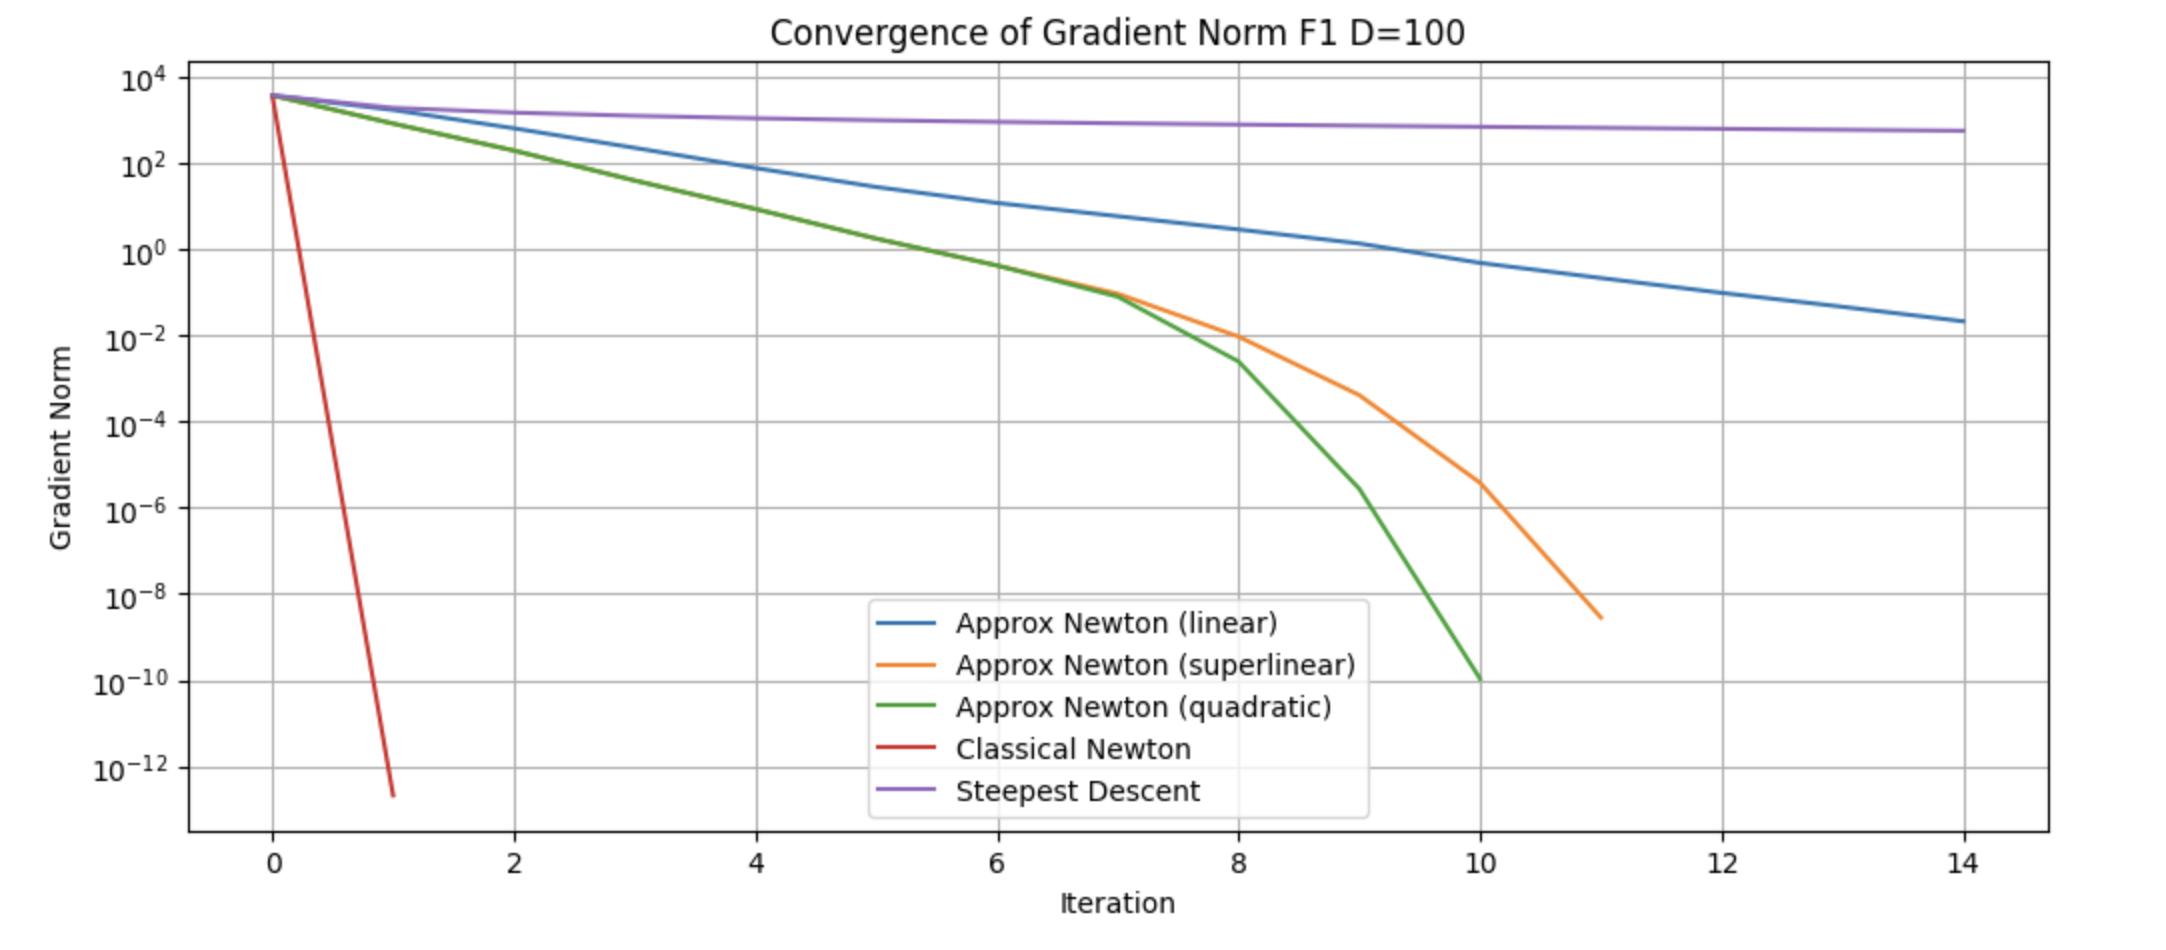
\includegraphics[width=0.8\textwidth]{pics/h3-1}
    \caption{Comparison of convergence rates under different $\eta$ schedules}
    \label{fig:convergence}
\end{figure}



\subsection{CG Step Efficiency}
\begin{itemize}
    \item Linear Approximate Newton uses fewer CG steps per iteration (~7.87), and trades accuracy per iteration for more iterations overall.
    \item Quadratic Convergence: there needs to be more CG iterations per step.
    \item Superlinear Convergence: Faster than linear but not as fast as quadratic.
\end{itemize}


\begin{table}[h]
    \centering
    \begin{tabular}{lccc}
        \toprule
        \textbf{$\eta_k$ Schedule} & \textbf{Iterations} & \textbf{Total CG Steps} & \textbf{CG Steps per Iteration} \\
        \midrule
        Linear & 15 & 118 & 7.87 \\
        Superlinear & 11 & 142 & 12.91 \\
        Quadratic & 10 & 130 & 13.00 \\
        \bottomrule
    \end{tabular}
    \caption{CG Step Analysis for Different $\eta_k$ Schedule in Approximate Newton Method}
    \label{tab:cg_steps}
\end{table}



\subsection{Method Comparison}
\begin{tabular}{llll}
    \toprule
    Metric & Approx. Newton & Classical Newton & Steepest Descent \\
    \midrule
    Convergence rate & Superlinear & Quadratic & Linear \\
    Computational cost & Medium & High & Low \\
    Memory requirements & Low & High & Low \\
    \bottomrule
\end{tabular}

\section{Discussion}
\subsection{Theoretical vs Empirical Observations}
\begin{itemize}
    \item Quadratic convergence achieved only with exact line search
    \item Superlinear convergence requires careful $\eta$ scheduling
    \item Dimension-dependent effects on CG performance
\end{itemize}

\subsection{Limitations}
\begin{itemize}
    \item Restricted to convex problems (Hessian constraints)
    \item Sensitivity to initial conditions
    \item Curse of dimensionality in high-$d$ regimes
\end{itemize}


\section{Conclusion}

Key findings:
\begin{itemize}
    \item Classical Newton performs well for the problem with cheap Hessians.
    \item Approximate Newton provides best balance for $d \geq 20$. 
    \item Adaptive $\eta$ scheduling crucial for optimal performance
    \item CG efficiency depends on spectrum of Hessian
\end{itemize}



\end{document}
